\section{Modelo de Negocio}
Para el desarrollo del modelo de negocio se implementó el modelo canva , el cual permite visualizar los aspectos fundamentales del modelo de negoccio del proyecto, estos son los socios claves que tendrá la empresa, actividades claves que realizará la empresa, propuestas de valor que tendrá la empresa, recursos clave para llevar a cabo las actividades, la estructurá de costos que manejará la empresa, las relaciones con el cliente que mantendrá la empresa, los canales por los cuales se moverá la empresa, las fuentes de ingresos que tendrá la empresa y los segmentos de clientes que tendrá la empresa.
Lo anteríor mencionado se ve ilustrado en la siguiente figura del modelo canva del proyecto
\begin{adjustbox}{
    center,
    caption=[{Modelo de negocio Canvas}]{\centering Modelo Canvas. Fuente:(Autores)},
    label={Modelo de negocio canvas},
    nofloat=figure}

    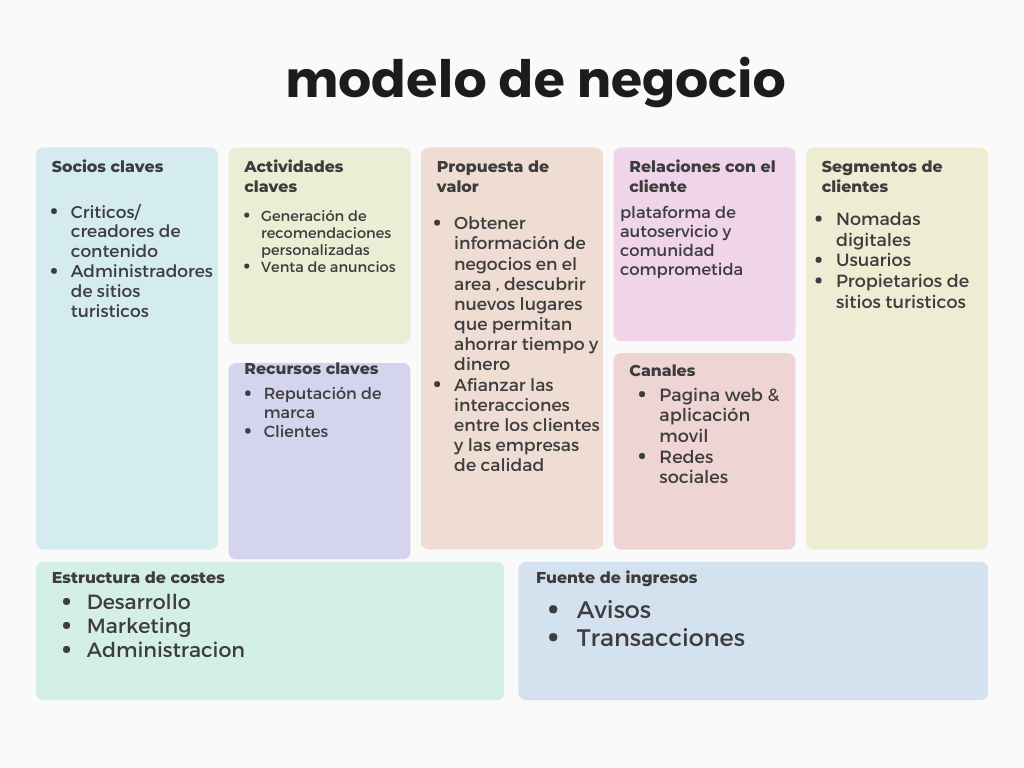
\includegraphics [scale=0.61]{Content/Images/Canva Emprendimiento.png}

\end{adjustbox}


\subsection{Segmento de clientes (SC)}
En esta sección se explora el segmento de clientes al que está enfocado el proyecto, en este caso los segmentos son los nomadas digitales en primer lugar, luego los usuarios generales del proyeto y por ultimo los propietarios de sitios turisticos que deseen ser parte del proyecto promocionandose.
\subsection{Propuesta de valor (PV)}
En esta sección se describen las propuestas de valor que permitirá el proyecto destacar entre los diferentes proveedores del mismo servicio, las propuestas de valor son la obtención de información de negocios en el area,descubrir nuevos lugares que permitan ahorrar dinero y tiempo al usuario final de la aplicación; Además de afianzar las interacciones entre los usuarios y las empresas que demuestren tener un servicio destacable.
\subsection{Canales de distribución (CD)}
En esta sección se especifican los canales de distribución del servicio que dará el proyecto , el principal es la pagina web y la aplicación movil en la que se desplegarán los servicios del proyecto, tambien se tienen en cuenta las redes sociales por ser el canal por el cual se publicitará el proyecto
\subsection{Relaciones con clientes (RCI)}
En esta sección se indican las relaciones que se tendrá con los clientes en la cual se explica que dicha relación será como una plataforma de autoservicio y comunidad comprometida para enriquecer la experiencia de los demás usuarios
\subsection{Fuentes de ingresos (FI)}
En esa sección están las fuentes de ingresos que tendrá el proyecto , las cuales son los avisos de diversos proveedores de servicios de turismo y transacciones al comprar cupones u ofertas que tengan los proveedores de servicios de turismo
\subsection{Recursos clave (RC)}
En esta sección se valoran los recursos clave del proyecto siendo estos la reputación de la marca ya que es fundamental que los usuarios tengan plena confianza en las recomendaciones brindadas, además de este los clientes son clave para que las recomendaciones esten bien fundamentadas en las experiencias de estos.
\subsection{Actividades clave (AC)}
En esta sección se presentan las actividades claves que tendrá el proyecto, estas son la generación de recomendaciones personalizadas, estas se basarán en la ubicación del usuario, en su presupuesto, en las calificaciones de otros usuarios y en las calificaciones pasadas del mismo usuario; además se tendrá la venta de anuncios de proveedores de servicios turisticos , incluso estas estan sujetas a las calificaciones de los usuarios, pero la venta de anuncios les permitirá a los proveedores darse a conocer
\subsection{Asociaciones o socios clave(AsC)}
En esta sección se posicionan los socios clave, comprendiendo a los criticos o creadores de contenido que permitirán dar a conocer el proyecto y esto enriquecerá el banco de recomendaciones mejorando así la calidad de las recomendaciones; tambien se tienen en cuenta los administradores de sitios turisticos ya que estos podrán promocionarse en el proyecto y asi mismo contribuir a aumentar la cantidad de usuarios.
\subsection{Estructura de costos (EC)}
En esta sección se indica la estructura de costes, donde destaca el desarrollo del proyecto, el marketing que se trabajará en el proyecto y la administración del proyecto.

\section{Esquema de ventas}
Un esquema de ventas es la estrategia estructurada que define cómo una empresa comercializa y vende sus productos o servicios. Este esquema establece los canales de distribución, el público objetivo, los procesos de captación de clientes, las fuentes de ingresos y las estrategias de conversión y fidelización.

En otras palabras, el esquema de ventas detalla cómo la empresa genera ingresos mediante un enfoque claro y organizado, asegurando que sus productos o servicios lleguen de manera efectiva a los clientes potenciales.

\subsection{Elementos clave de un esquema de ventas:}
\begin{itemize}
   \item Segmentación del mercado: Identificación de clientes ideales.

\item Propuesta de valor: Beneficio único del producto o servicio.

\item Fuentes de ingresos: Métodos de monetización.

\item Canales de ventas: Medios para atraer y cerrar ventas (online/offline).

\item Estrategias de conversión: Métodos para transformar clientes potenciales en compradores.

\item Fidelización del cliente: Acciones para mantener y retener clientes.
\end{itemize}


\subsection{Esquema de ventas aplicado}

\begin{itemize}
    \item Segmentación del mercado:
    \begin{itemize}
    \item Nómadas digitales que buscan destinos seguros y confiables.
    \item Turistas extranjeros y nacionales interesados en experiencias seguras.
    \item Empresas turísticas (hoteles, coworkings, restaurantes, agencias de tours) que deseen posicionar sus servicios con un enfoque en seguridad.
    \end{itemize}
    \item Propuesta de valor:
    \begin{itemize}
        \item Plataforma confiable con reseñas verificadas por usuarios y moderadores, garantizando información actualizada y transparente.
        \item Sistema de recomendación basado en IA para sugerencias personalizadas según perfil, intereses y ubicación del usuario.
        \item Mapeo interactivo de zonas seguras y alertas en tiempo real sobre riesgos en ciertas áreas, permitiendo una toma de decisiones informada.

    \end{itemize}
    \item Fuentes de ingresos:
    \begin{itemize}
        \item Suscripción Premium para usuarios: Acceso a recomendaciones más detalladas, alertas en tiempo real y funciones avanzadas.
        \item Publicidad y asociaciones con negocios locales: Hoteles, restaurantes y espacios de coworking pagan por visibilidad en la plataforma.
    \end{itemize}
    
   \item Canales de ventas:
    \begin{itemize}
        \item Plataforma web y aplicación móvil.
        \item Marketing digital (SEO, SEM, redes sociales, influencers nómadas).
        \item Alianzas con embajadas y asociaciones de nómadas digitales.
    \end{itemize}
   \item Estrategia de conversión y fidelización:
    \begin{itemize}
        \item Pruebas gratuitas de funcionalidades premium.
        \item Descuentos y beneficios exclusivos para suscriptores.
    \end{itemize}
\end{itemize} 
